\documentclass[10pt,a4paper]{beamer}
\usepackage[utf8]{inputenc}
\usepackage{amsmath}
\usepackage{amsfonts}
\usetheme{Berkeley}
\usepackage{amssymb}
\usepackage{graphicx}
\author{Richard Torenvliet}
\title{Flood Simulation Browser}
\begin{document}
\begin{frame}
\maketitle
\end{frame}
\section{Introductie}
\begin{frame}
\frametitle{Introduction}
\begin{columns}[c]
\column{1.5in}
\begin{itemize}
\item Urban Flood Project
\item Early Warning System
\item Burgers en Hulpdiensten
\item Sensoren in dijk + Internet
\item Water Simulatie
\item Hoogte Kaart
\end{itemize}
\column{2.0in}
\begin{figure}
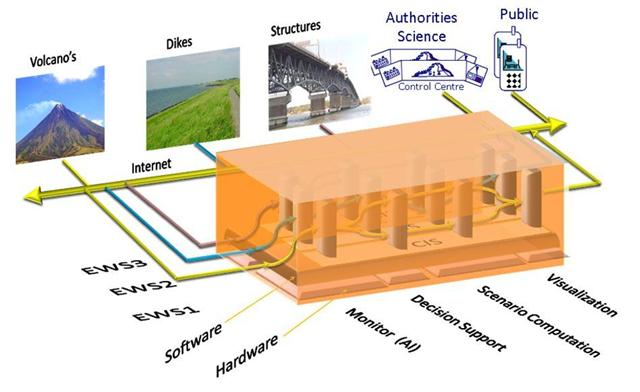
\includegraphics[scale=0.3]{concept.png}
\caption{Bron: \url{http://urbanflood.eu/aboutus.aspx}}
\end{figure}
\end{columns}
\end{frame}
\section{Doel Flood Simulation Browser}
\begin{frame}
\frametitle{Doel Flood Simulation Browser}
\begin{columns}[c]
\column{5cm}
\begin{itemize}
\item Visualisatie laten zien
\item Informeren over overstromingsgebied
\item Zien wat er als eerst onderwater gaat
\item Evacuatie routes
\item Hulpdienst routes
\item Browse door alle simulaties
\item Nieuwe simulatie uitvoeren
\end{itemize}
\column{5cm}
\begin{figure}
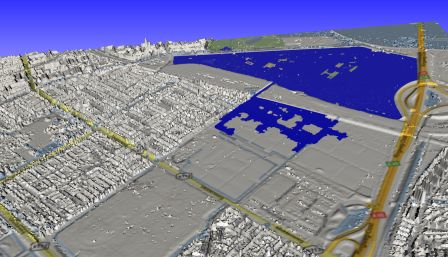
\includegraphics[scale=0.5]{simulation.png}
\caption{Bron: \url{http://urbanflood.eu/default.aspx}}
\end{figure}
\end{columns}
\end{frame}
\section{Mijn Doel}
\begin{frame}
\frametitle{Mijn Doel}
\begin{itemize}
\item Browser geschikt maken voor Tablets
\item \textbf{Geen} water simuleren
\item Server levert plaatjes + coördinaten
\item Plaatjes over Google maps leggen - uitgebreid API support voor overlays
\item Intuïtief design
\item Taal/framework keuze
\item Mijn eis is: Crossplatform
\end{itemize}
\end{frame}
\section{Reeds gedaan}
\begin{frame}
\frametitle{Reeds Gedaan}
\begin{itemize}
\item Alle mogelijkheden afgegaan
\begin{itemize}
\item iOS Objective C - niet crossplatform - hoge leercurve
\item Android Java - idem
\item jQuery Mobile - Niet gemoduleerd, combinatie PhoneGap
\item Titanium - Makkelijk, maar vrij groot, Veel geheugen gebruik, Design anders op andere telefoons en niet ECHT crossplatform
\end{itemize}
\item Platform keuze gemaakt
\item Sencha Touch 2 ervaring opgedaan
\item Voordelen
\begin{itemize}
\item Crossplatform
\item MVC Design Pattern
\item Mobiele website of App
\item Android en iOS
\item Geen PhoneGap nodig
\end{itemize}
\item Nadelen
\begin{itemize}
\item Verschilt veel met huidige persoonlijke kennis webtechnologiën
\item Highlevel specificatie
\item Mogelijk onvoorziene problemen
\end{itemize}
\end{itemize}
\end{frame}
\section{Referenties}
\begin{frame}
\begin{thebibliography}{9}
\frametitle{Referenties}
\bibitem{urban flood}
  Urban Flood Project,
  \url{http://urbanflood.eu/default.aspx}.
  Retrieved 9 april
\bibitem{Sencha Touch}
	Sencha Touch 2.
	\url{http://docs.sencha.com/touch/2-0/}.
	Retrieved 9 april
\bibitem{Google Maps API}
	Google Maps API,
	\url{https://developers.google.com/maps/}.
	Retrieved 9 april
\bibitem{PhoneGap}
	PhoneGap
	\url{http://www.PhoneGap.com}.
	Retrieved 9 april
\bibitem{Titanium Mobile}
	Titanium Appcelerator,
	\url{http://www.appcelerator.com/}.
	Retrieved 9 april
\end{thebibliography}
\end{frame}
\end{document}